\documentclass{standalone}
\usepackage{tikz}
\usetikzlibrary{patterns, positioning}
\usetikzlibrary{shapes.misc}
\usepackage[outline]{contour}
\contourlength{1.5pt} 
\usepackage[sfdefault]{ClearSans} %% option 'sfdefault' activates Clear Sans as the default text font
\usepackage[T1]{fontenc}

\begin{document}
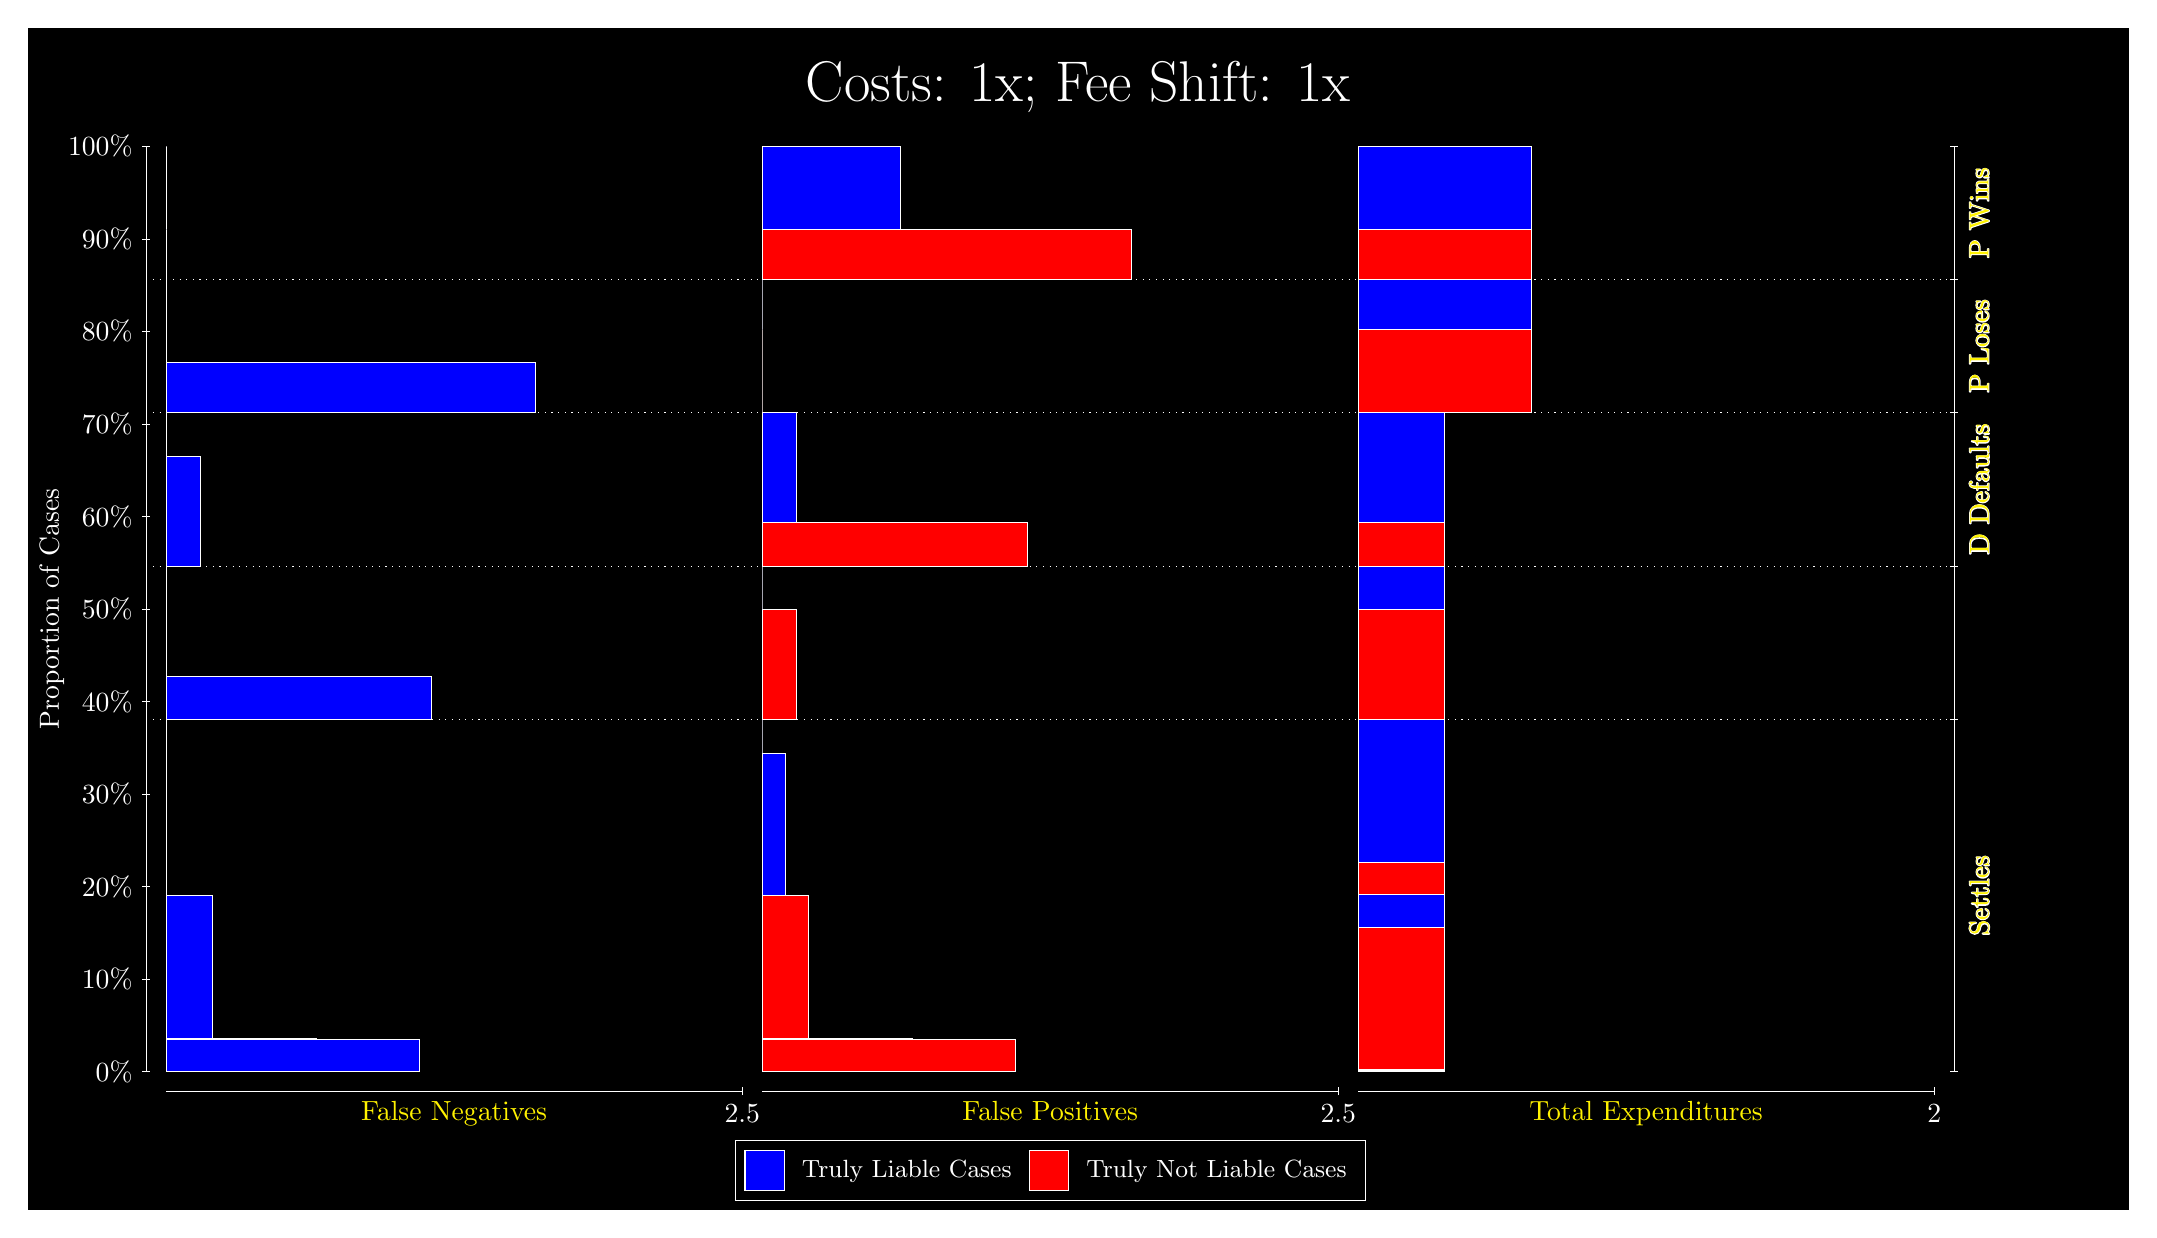
\begin{tikzpicture}
\draw[fill=black] (0,0) rectangle (26.667,15);
\draw[text=white] (0,13.5) rectangle (26.667,15) node[midway] {\huge Costs: 1x; Fee Shift: 1x};
\draw[white, very thin] (1.5,1.75) -- (1.5,13.5);
\node[rotate=90, text=white, anchor=center] at (0.3, 7.625) {Proportion of Cases};
\draw[white, very thin] (1.45,1.75) -- (1.55,1.75);
\node[text=white, anchor=east] at (1.45, 1.75) {0\%};
\draw[white, very thin] (1.45,2.925) -- (1.55,2.925);
\node[text=white, anchor=east] at (1.45, 2.925) {10\%};
\draw[white, very thin] (1.45,4.1) -- (1.55,4.1);
\node[text=white, anchor=east] at (1.45, 4.1) {20\%};
\draw[white, very thin] (1.45,5.275) -- (1.55,5.275);
\node[text=white, anchor=east] at (1.45, 5.275) {30\%};
\draw[white, very thin] (1.45,6.45) -- (1.55,6.45);
\node[text=white, anchor=east] at (1.45, 6.45) {40\%};
\draw[white, very thin] (1.45,7.625) -- (1.55,7.625);
\node[text=white, anchor=east] at (1.45, 7.625) {50\%};
\draw[white, very thin] (1.45,8.8) -- (1.55,8.8);
\node[text=white, anchor=east] at (1.45, 8.8) {60\%};
\draw[white, very thin] (1.45,9.975) -- (1.55,9.975);
\node[text=white, anchor=east] at (1.45, 9.975) {70\%};
\draw[white, very thin] (1.45,11.15) -- (1.55,11.15);
\node[text=white, anchor=east] at (1.45, 11.15) {80\%};
\draw[white, very thin] (1.45,12.325) -- (1.55,12.325);
\node[text=white, anchor=east] at (1.45, 12.325) {90\%};
\draw[white, very thin] (1.45,13.5) -- (1.55,13.5);
\node[text=white, anchor=east] at (1.45, 13.5) {100\%};

\draw[white, very thin] (24.457,1.75) -- (24.457,13.5);
\draw[white, very thin] (24.407,1.75) -- (24.507,1.75);
\node[anchor=west] at (24.407, 1.75) {};
\draw[white, very thin] (24.407,6.2206) -- (24.507,6.2206);
\node[anchor=west] at (24.407, 6.2206) {};
\draw[white, very thin] (24.407,8.1688) -- (24.507,8.1688);
\node[anchor=west] at (24.407, 8.1688) {};
\draw[white, very thin] (24.407,10.117) -- (24.507,10.117);
\node[anchor=west] at (24.407, 10.117) {};
\draw[white, very thin] (24.407,11.809) -- (24.507,11.809);
\node[anchor=west] at (24.407, 11.809) {};
\draw[white, very thin] (24.407,13.5) -- (24.507,13.5);
\node[anchor=west] at (24.407, 13.5) {};

\draw[white, very thin, fill=blue] (1.75,1.75) rectangle (4.9703,2.1614);
\draw[white, very thin, fill=blue] (1.75,2.1614) rectangle (3.6529,2.1741);
\draw[white, very thin, fill=blue] (1.75,2.1741) rectangle (2.3355,3.9852);
\draw[white, very thin, fill=red] (1.75,3.9852) rectangle (1.75,6.2206);
\draw[white, very thin, fill=blue] (1.75,6.2206) rectangle (5.1167,6.7748);
\draw[white, very thin, fill=red] (1.75,6.7748) rectangle (1.75,8.1688);
\draw[white, very thin, fill=blue] (1.75,8.1688) rectangle (2.1891,9.5628);
\draw[white, very thin, fill=red] (1.75,9.5628) rectangle (1.75,10.117);
\draw[white, very thin, fill=blue] (1.75,10.117) rectangle (6.4341,10.754);
\draw[white, very thin, fill=red] (1.75,10.754) rectangle (1.75,11.809);
\draw[white, very thin, fill=red] (1.75,11.809) rectangle (1.75,12.445);
\draw[white, very thin, fill=blue] (1.75,12.445) rectangle (1.75,13.5);
\draw[white, very thin, fill=red] (9.3189,1.75) rectangle (12.539,2.1613);
\draw[white, very thin, fill=red] (9.3189,2.1613) rectangle (11.222,2.174);
\draw[white, very thin, fill=red] (9.3189,2.174) rectangle (9.9044,3.9854);
\draw[white, very thin, fill=blue] (9.3189,3.9854) rectangle (9.6116,5.7966);
\draw[white, very thin, fill=blue] (9.3189,5.7966) rectangle (9.3189,6.2206);
\draw[white, very thin, fill=red] (9.3189,6.2206) rectangle (9.758,7.6146);
\draw[white, very thin, fill=blue] (9.3189,7.6146) rectangle (9.3189,8.1688);
\draw[white, very thin, fill=red] (9.3189,8.1688) rectangle (12.686,8.723);
\draw[white, very thin, fill=blue] (9.3189,8.723) rectangle (9.758,10.117);
\draw[white, very thin, fill=red] (9.3189,10.117) rectangle (9.3189,11.172);
\draw[white, very thin, fill=blue] (9.3189,11.172) rectangle (9.3189,11.809);
\draw[white, very thin, fill=red] (9.3189,11.809) rectangle (14.003,12.445);
\draw[white, very thin, fill=blue] (9.3189,12.445) rectangle (11.075,13.5);
\draw[white, very thin, fill=red] (16.888,1.75) rectangle (17.986,1.7627);
\draw[white, very thin, fill=blue] (16.888,1.7627) rectangle (17.986,1.7754);
\draw[white, very thin, fill=red] (16.888,1.7754) rectangle (17.986,3.5868);
\draw[white, very thin, fill=blue] (16.888,3.5868) rectangle (17.986,3.9982);
\draw[white, very thin, fill=red] (16.888,3.9982) rectangle (17.986,4.4095);
\draw[white, very thin, fill=blue] (16.888,4.4095) rectangle (17.986,6.2206);
\draw[white, very thin, fill=red] (16.888,6.2206) rectangle (17.986,7.6146);
\draw[white, very thin, fill=blue] (16.888,7.6146) rectangle (17.986,8.1688);
\draw[white, very thin, fill=red] (16.888,8.1688) rectangle (17.986,8.723);
\draw[white, very thin, fill=blue] (16.888,8.723) rectangle (17.986,10.117);
\draw[white, very thin, fill=red] (16.888,10.117) rectangle (19.083,11.172);
\draw[white, very thin, fill=blue] (16.888,11.172) rectangle (19.083,11.809);
\draw[white, very thin, fill=red] (16.888,11.809) rectangle (19.083,12.445);
\draw[white, very thin, fill=blue] (16.888,12.445) rectangle (19.083,13.5);
\draw[white, dotted] (1.5,6.2206) -- (24.457,6.2206);
\draw[white, dotted] (1.5,8.1688) -- (24.457,8.1688);
\draw[white, dotted] (1.5,10.117) -- (24.457,10.117);
\draw[white, dotted] (1.5,11.809) -- (24.457,11.809);
\draw[white, very thin] (1.75,1.5) -- (9.0689,1.5);
\node[text=yellow, anchor=north] at (5.4094, 1.5) {False Negatives};
\draw[white, very thin] (9.0689,1.45) -- (9.0689,1.55);
\node[text=white, anchor=north] at (9.0689, 1.45) {2.5};

\draw[white, very thin] (9.3189,1.5) -- (16.638,1.5);
\node[text=yellow, anchor=north] at (12.978, 1.5) {False Positives};
\draw[white, very thin] (16.638,1.45) -- (16.638,1.55);
\node[text=white, anchor=north] at (16.638, 1.45) {2.5};

\draw[white, very thin] (16.888,1.5) -- (24.207,1.5);
\node[text=yellow, anchor=north] at (20.547, 1.5) {Total Expenditures};
\draw[white, very thin] (24.207,1.45) -- (24.207,1.55);
\node[text=white, anchor=north] at (24.207, 1.45) {2};

\node[text=yellow, centered, rotate=90] at (24.777, 3.9853) {\contour{white}{Settles}};

\node[text=yellow, centered, rotate=90] at (24.777, 9.1429) {\contour{white}{D Defaults}};
\node[text=yellow, centered, rotate=90] at (24.777, 10.963) {\contour{white}{P Loses}};
\node[text=yellow, centered, rotate=90] at (24.777, 12.654) {\contour{white}{P Wins}};

\draw (12.978300999999998,1.5) node[draw=none] (baseCoordinate) {};
\begin{scope}[align=center]
        \matrix[scale=0.5, draw=white, below=0.5cm of baseCoordinate, nodes={draw}, column sep=0.1cm]{
            \node[rectangle, draw, minimum width=0.5cm, minimum height=0.5cm, fill=blue] {}; &
            \node[draw=none, font=\small, text=white] (B) {Truly Liable Cases}; &
            \node[rectangle, draw, minimum width=0.5cm, minimum height=0.5cm, fill=red] {}; &
            \node[draw=none, font=\small, text=white] (B) {Truly Not Liable Cases}; \\
            };
\end{scope}

\end{tikzpicture}
\end{document}